\documentclass[a4paper,11pt]{article}

% Identificação
\newcommand{\pbtitulo}{Flume}
\newcommand{\pbversao}{1.0}

\usepackage{../../sty/tutorial}

%----------------------------------------------------------------------
% Início do Documento
%----------------------------------------------------------------------
\begin{document}
	
	\maketitle % mostrar o título
	\thispagestyle{fancy} % habilitar o cabeçalho/rodapé das páginas
	
%--------------------------------------------------------------------------
% RESUMO DO ARTIGO
%--------------------------------------------------------------------------
\begin{abstract}
	% O primeiro caractere deve vir com \initial{}
	\initial{F}lume\cite{flumeoficial} ou "Apache Flume" (aqui chamarei apenas de Flume) é parte do Ecosistema Hadoop criado para ser um sistema confiável e distribuído para coletar, agregar e mover grandes quantidades de dados de registros (Log), eventos, dados de redes sociais ou sensores para um armazenamento de dados centralizados como o \textbf{HBase} ou \textbf{HDFS} para posterior análise. Possui uma arquitetura simples, porém flexível, baseada em fluxos de dados de streaming.
\end{abstract}

%--------------------------------------------------------------------------
% CONTEÚDO DO ARTIGO
%--------------------------------------------------------------------------
\section{Parte inicial}
Flume é uma ferramenta para alimentação de dados em HDFS. Acumula, integra e transporta grandes quantidades de dados de \textit{streaming}, como arquivos de log, eventos de diferentes origens, como tráfego de rede, mensagens de e-mail para o \textbf{HDFS}. Flume é altamente confiável e distribuído. 
\begin{figure}[H]
	\centering
	
\includegraphics[width=0.5\textwidth]{imagem/logo}
	\caption{Logo do Apache Flume}
\end{figure}

Flume tem um design flexível baseado em fluxos de dados de \textit{streaming}. É tolerante a falhas e robusto com vários \textit{failovers} (tratamento de exceção) e mecanismos de recuperação. O \textbf{Flume Big Data} tem diferentes níveis de confiabilidade para oferecer, que incluem \textit{best-effort delivery} (entrega com o melhor esforço) e \textit{end-to-end delivery} (entrega de ponta a ponta). \textit{Best-effort delivery} não tolera nenhuma falha de nó do Flume, enquanto o modo \textit{end-to-end delivery} garante a entrega mesmo no caso de várias falhas de nó.

Flume transporta dados entre fontes e coletores. Essa coleta de dados pode ser agendada ou orientada a eventos. O Flume tem seu próprio mecanismo de processamento de consultas que facilita a transformação de cada novo lote de dados antes de serem movidos para o coletor pretendido.

Possíveis coletores Flume incluem \textbf{HDFS} e \textbf{HBase}. O Flume Hadoop também pode ser usado para transportar dados de eventos, incluindo, entre outros, dados de tráfego de rede, dados gerados por sites de mídia social e mensagens de e-mail.

Estes são os benefícios que o tornam uma alternativa melhor em relação aos outros: \vspace{-1em}
\begin{itemize}
	\item É tolerante a falhas, confiável e escalável.
	\item Pode armazenar dados em locais centralizados como HBase e HDFS.
	\item Escalável horizontalmente.
	\item Se a taxa de leitura ultrapassar a taxa de gravação, o Flume fornecerá um fluxo
	constante de dados entre a leitura e a gravação de dados.
	\item A entrega de mensagens é confiável. As transações são baseadas em canal; para cada mensagem, duas transações são mantidas.
	\item Sustenta um conjunto abrangente de tipos de origens e destinos.
	\item Dados de várias fontes podem ser ingeridos no Hadoop.
\end{itemize}

\section{Arquitetura do Flume}
Um agente Flume é um processo independente que roda por trás de uma JVM (\textit{Java Virtual Machine}), possui 3 componentes: \textbf{Flume Source}, \textbf{Flume Channel} e \textbf{Flume Sink}. Através dos quais os eventos se propagam após serem iniciados em uma fonte externa:
\begin{figure}[H]
	\centering
	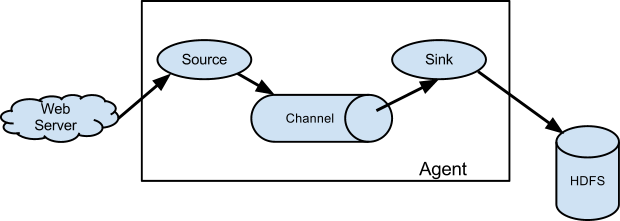
\includegraphics[width=0.8\textwidth]{imagem/arquitetura}
	\caption{Arquitetura do Apache Flume}
\end{figure}

Na imagem vemos como os componentes se comportam: \vspace{-1em}
\begin{itemize}
	\item Os eventos gerados pela fonte externa (\textit{WebServer}) são consumidos pelo \textbf{Flume Source}. A fonte externa envia eventos para a fonte Flume em um formato que é reconhecido pela fonte de destino.
	\item \textbf{Flume Source} recebe um evento e o armazena em um ou mais canais através do \textbf{Flume Channel}. Atua como um armazenamento transitório e mantém o evento até que seja consumido pelo \textbf{Flume Sink}. Este também pode utilizar um sistema de arquivos local para armazenar esses eventos.
	\item \textbf{Flume Sink} remove o evento de um canal e o armazena em um repositório externo como, por exemplo, \textbf{HDFS}. Pode haver vários agentes do Flume, caso no qual \textbf{Flume Sink} encaminha este evento para o próximo agente no fluxo.
\end{itemize}

Definições do Flume: \vspace{-1em}
\begin{itemize}
	\item \textbf{Event} (evento) - É a menor unidade de dados que transita no Flume.
	\item \textbf{Header} (cabeçalho) - É a parte opcional de \textit{Event} ou do dado em si (denominado de \textit{Payload}).
\end{itemize}
\begin{figure}[H]
	\centering
	
\includegraphics[width=0.5\textwidth]{imagem/event}
	\caption{Definições da Arquitetura do Flume}
\end{figure}

Exemplos de soluções com o Flume: \vspace{-1em}
\begin{itemize}
	\item \textbf{Facebook Scribe} - \textbf{Scribe} é uma ferramenta usada para agregar e transmitir dados de log. Projetado para dimensionar um número muito grande de nós e extremamente robusto a falhas de nós e de rede.
	\item Apache Kafka - desenvolvido pela \textbf{ASF} (\textit{Apache Software Foundation}) como um agente de mensagens de código aberto. Com o Kafka podemos lidar com \textit{feeds} através de alta transferência (\textit{high-throughput}) e baixa latência.
\end{itemize}

\section{Hadoop no Docker}
O modo mais simples de se conseguir trabalhar com o Hadoop é utilizando o Docker, para baixar a imagem do Hadoop: \\
\codigo{\$ docker pull suhothayan/hadoop-spark-pig-hive:2.9.2}

Nessa imagem temos outros produtos do Ecossistema Hadoop: Spark, Pig e Hive. Para criar e executar a primeira vez o contêiner (a pasta que este comando for executado será associada a uma pasta interna chamada \textbf{/home/tsthadoop}): \\
\codigo{\$ docker run -it -d --name meu-hadoop -v \$(pwd):/home/tsthadoop \\ suhothayan/hadoop-spark-pig-hive:2.9.2}

Uma vez interrompido o contêiner: \\
\codigo{\$ docker stop meu-hadoop}

Podemos executá-lo novamente com os seguintes comandos: \\
\codigo{\$ docker start meu-hadoop \\
\$ docker exec -it meu-hadoop /etc/bootstrap.sh bash}

\subsection{Erro de Permissão}
Na primeira vez que entramos é dado um erro na execução do script "bootstrap.sh" de permissão negada para executar o script "spark-env.sh", vamos corrigir isso com o comando: \\
\codigo{\# chmod 777 /usr/local/spark/conf/spark-env.sh}

Vamos sair do bash: \\
\codigo{\# exit}

Podemos executá-lo novamente: \\
\codigo{\$ docker exec -it meu-hadoop /etc/bootstrap.sh bash}

E o erro desapareceu.


E podemos verificar a versão do Hadoop está instalado: \\
\codigo{\$ hadoop version}

\subsection{Instalar o Flume}
Se leu corretamente essa imagem NÃO POSSUI o \textbf{Flume} e agora realmente começa nossa instalação, optei por utilizar essa imagem por já possuir todos os componentes necessários para posterior tratamento dos dados. Desta forma ao invés de realizar um trabalho de obter uma imagem somente com o Flume (que existem várias por aí e ter que instalar todos os outros componentes), vamos utilizar uma imagem que estamos acostumados e que já possui todas as outras ferramentas necessárias e nos preocuparmos apenas com o \textbf{Flume}.

Outros ganhos adicionais desse método, é ser excelente para aprendermos como adicionar uma ferramenta ao ecossistema do \textbf{Hadoop}, além de não ficarmos presos a uma determinada versão. E agora podemos "brincar" melhor com as outras ferramentas como o \textbf{Spark}, \textbf{Hive} e \textbf{Pig} que já estão nessa imagem (e se já utilizou o tutorial sobre \textbf{Sqoop} verá que este também já se encontra instalado).

No endereço oficial \cite{flumeoficial} existe o link para \textit{download}, e ao acessar este temos as versões disponíveis do \textbf{Flume}. Utilizaremos a última até o momento, clicar no link "1.9.0" e baixar o arquivo \textbf{apache-flume-1.9.0-bin.tar.gz} e colocá-lo na pasta associativa da imagem.

Retornar a pasta raiz do root: \\
\codigo{\# cd root/}

Descompactar o arquivo: \\
\codigo{\# tar vfx /home/tsthadoop/apache-flume-1.11.0-bin.tar.gz}

Mover o pasta descompactada para o endereço local (aonde estão os outros produtos do Ecossistema): \\
\codigo{\# mv apache-flume-1.11.0-bin /usr/local/.}

Criar um link simbólico para facilitar o acesso: \\
\codigo{\# cd /usr/local/} \\
\codigo{\# ln -s /usr/local/apache-flume-1.11.0-bin flume}

Modificar o arquivo "etc/bootstrap.sh":
\codigo{\# vim /etc/bootstrap.sh}

E adicionar as seguintes linhas abaixo dos comandos EXPORT:
\begin{lstlisting}[]
export FLUME_HOME="/usr/local/flume"
export PATH=$PATH:/usr/local/sqoop/bin:/usr/local/flume/bin
\end{lstlisting}

Aproveitamos e inserimos o caminha do path para a pasta do Flume (considerando que já existe a do Sqoop). Pressionar "ESC" para sair do modo de edição e salvar o arquivo com ”:wq”. Sair da imagem, parar e iniciar o contêiner, entrar no bash novamente. Acessar a pasta associativa: \\
\codigo{\# cd /home/tsthadoop}

Verificar se o Flume está correto: \\
\codigo{\# flume-ng version}

\subsection{Trazer os dados}
Toda a brincadeira com o Flume se resume a um simples arquivo contendo os dados que ele irá levar diretamente para o HDFS, consideremos para este exemplo um simples arquivo texto contido na pasta associativa chamado "familia.txt", com o seguinte conteúdo:
\begin{lstlisting}[]
Fernando,Anselmo
Jessica,Rabbit
Robin,Batman
Hugo,Anselmo
Roger,Rabbit
Fox,Rabbit
Bruce,Batman
\end{lstlisting}

Nosso primeiro passo é criar um agente de configuração que observe esses dados, para tanto, na pasta "/usr/local/flume/conf" criamos um arquivo chamado "familia.conf":
\codigo{\# vim familia.conf}

E definimos as seguintes características:
\begin{lstlisting}[]
agent1.sources = tail
agent1.channels = Channel-2
agent1.sinks = sink-1

agent1.sources.tail.type = exec
agent1.sources.tail.command = cat /home/tsthadoop/familia.txt
agent1.sources.tail.channels = Channel-2

agent1.channels.Channel-2.type = memory

agent1.sinks.sink-1.channel = Channel-2
agent1.sinks.sink-1.type = hdfs
agent1.sinks.sink-1.hdfs.path = hdfs://localhost:9000/flume01
agent1.sinks.sink-1.hdfs.fileType = DataStream
agent1.sinks.sink-1.hdfs.useLocalTimeStamp = false
agent1.sinks.sink-1.hdfs.rollInterval = 60
agent1.sinks.sink-1.hdfs.round = true
agent1.sinks.sink-1.hdfs.roundValue = 10
agent1.sinks.sink-1.hdfs.roundUnit = second
\end{lstlisting}

Pressionar "ESC" para sair do modo de edição e salvar o arquivo com ”:wq”. Executamos o agente com o comando: \\
\codigo{\# flume-ng agent –conf /usr/local/flume/conf/ -f /usr/local/flume/conf/familia.conf -n agent1 -Dflume.root.logger=DEBUG,console}

Esse comando executa o Flume para verificar o arquivo e trazer os dados contidos nele, ao recebermos uma mensagem tal como:
\codigo{2022-12-19T19:44:05,631 INFO [hdfs-sink-1-call-runner-3] org.apache.flume.sink.hdfs.BucketWriter - Renaming hdfs://localhost:9000/flume01/FlumeData.1671475952091.tmp to hdfs://localhost:9000/flume01/FlumeData.1671475952091}

Significa que os dados já foram importados, damos um CTRL+C para interromper. Agora vamos ver se está tudo correto com o seguinte comando para verificar as pastas do HDFS: \\
\codigo{\# hdfs dfs -ls /}

Que mostra algo como: \\
\codigo{Found 3 items \\
drwxr-xr-x   - root supergroup          0 2022-12-19 18:53 /flume01 \\
drwx-wx-wx   - root supergroup          0 2022-12-19 17:59 /tmp \\
drwxr-xr-x   - root supergroup          0 2019-07-21 16:09 /user}

Se verificarmos a pasta criada pelo Flume: \\
\codigo{\# hdfs dfs -ls /flume01}

Teremos como resposta (obviamente o número final no arquivo pode variar): \\
\codigo{Found 1 items \\
-rw-r--r--   1 root supergroup         95 2022-12-19 18:53 /flume01/FlumeData.1671475952091}

E podemos verificar seu conteúdo: \\
\codigo{\# hdfs dfs -cat /flume01/FlumeData.1671475952091}

Que é exatamente igual aos dados que temos no arquivo original. Mais detalhes sobre as configurações dos canais podem ser acessadas aqui: \url{	https://flume.apache.org/releases/content/1.6.0/FlumeUserGuide.html}

Mais fontes de informação podem ser obtidas em diversos sites que apresenta tutoriais completos sobre o Apache Flume como a Tutorials Point\cite{tutorialspoint}.
	
\section{Conclusão}
Flume é uma ferramenta no ecossistema Hadoop que fornece recursos para coletar, agregar e trazer de forma eficiente grandes quantidades de dados para o Hadoop. Exemplos de grandes quantidades de dados são dados de log, dados de tráfego de rede, dados de mídia social, dados de geolocalização, dados de sensores e máquinas e dados de mensagens de e-mail. 

Fornece vários recursos para gerenciar dados e permite que os usuários absorvam de várias fontes de dados no Hadoop. Protege os sistemas contra picos de dados quando a taxa de entrada de dados excede a taxa na qual os dados são gravados. O Flume NG garante a entrega de dados usando transações baseadas em canal. É dimensionado horizontalmente para processar mais fluxos de dados e volumes de dados.

Geralmente é usado para dados de log. O Flume pode obter dados de várias fontes como Avro, Syslog’s e arquivos e os entrega para vários destinos como Hadoop HDFS ou HBase. Por ser basicamente um sistema distribuído usado para agregar os arquivos em um único local. Em termos simples, é usado para mover os dados de um local para outro de maneira confiável e eficiente. Possui recursos integrados, como mecanismos de confiabilidade, failover e recuperação, e é tolerante a falhas. É um componente importante no ecossistema Hadoop.

Sou um entusiasta do mundo \textbf{Open Source} e novas tecnologias. Qual a diferença entre Livre e Open Source? \underline{Livre} significa que esta apostila é gratuita e pode ser compartilhada a vontade. \underline{Open Source} além de livre todos os arquivos que permitem a geração desta (chamados de arquivos fontes) devem ser disponibilizados para que qualquer pessoa possa modificar ao seu prazer, gerar novas, complementar ou fazer o que quiser. Os fontes da apostila (que foi produzida com o LaTex) está disponibilizado no GitHub \cite{github}. Veja ainda outros artigos que publico sobre tecnologia através do meu Blog Oficial \cite{fernandoanselmo}.

%--------------------------------------------------------------------------
% REFERÊNCIAS
%--------------------------------------------------------------------------
\begin{thebibliography}{4}
	\bibitem{flumeoficial} 
	Página do Apache Flume \\
	\url{https://flume.apache.org}

	\bibitem{tutorialspoint} 
	Tutorials Point sobre Flume \\
	\url{https://www.tutorialspoint.com/apache_flume/index.htm}
	
		\bibitem{fernandoanselmo} 
	Fernando Anselmo - Blog Oficial de Tecnologia \\
	\url{http://www.fernandoanselmo.blogspot.com.br/}
	
	\bibitem{publicacao} 
	Encontre essa e outras publicações em \\
	\url{https://cetrex.academia.edu/FernandoAnselmo}
	
	\bibitem{github} 
	Repositório para os fontes da apostila \\
	\url{https://github.com/fernandoans/publicacoes}
\end{thebibliography}

\end{document}